\documentclass[t]{beamer}
\setlength{\parskip}{5pt}
%\usetheme{Madrid}  

\usepackage[UKenglish]{babel}
\usepackage[UKenglish]{isodate}
\cleanlookdateon

%\usepackage{listings}
\usepackage{tikz}
\usepackage{graphicx}

\newtheorem{remark}{Remark}

\def\le{\leqslant}
\def\ge{\geqslant}

\def\Z{\mathbb{Z}}
\def\N{\mathbb{N}}
\def\R{\mathbb{R}}
\def\C{\mathbb{C}}
\def\Q{\mathbb{Q}}

\title{CS3230 Tutorial 7}
\author{Deng Tianle (T15)}
\date{10 October 2025}

\begin{document}

\frame{\titlepage} 

\begin{frame}{Greedy algorithms}
  Greedy algorithms solve problems that have optimal substructure and greedy choice property. 
  \par Optimal substructure: same as in DP; optimal is obtained by piecing together optimal solutions for subproblems. 
  \par Greedy choice property: local optimal choices lead to \textbf{a} global optimal
  \par The concepts and proofs are illustrated by the problems we will discuss. 
\end{frame}
\begin{frame}{Burning CDs problem}
  Consider a set of files $\{f_1, \dots, f_n\}$ where each $f_i$ has size $<100$. We want to store all files into CDs that each has capacity $100$. Each file must be stored in a single CD (cannot be split), and each CD can store \textbf{at most $2$} files. 
\end{frame}
\begin{frame}{Q1 (Optimal substructure)}
  Assume there exists a pair of files that fit into one CD. 
  \begin{enumerate}
    \item For any $f_1, f_2$, $MinCD(A) = 1 + MinCD(A-\{f_1, f_2\})$? No: say $A = \{1, 45, 45, 90\}$, then $MinCD(A)=2 < 1+MinCD(\{45, 90\})$. 
    \item Now suppose $f_1, f_2$ belongs to a single CD in an optimal solution. Then yes, $MinCD(A) = 1 + MinCD(A-\{f_1, f_2\})$. This is because for an optimal solution with $f_1, f_2$ on the same CD, the arrangement for the other files/CDs must be optimal (otherwise there will be a better solution, contradiction). 
    \item If $f_1, f_2$ is largest and smallest file respectively then still no, because they may not even fit into one CD. 
  \end{enumerate}
\end{frame}
\begin{frame}{Q2 (Greedy choice)}
  Assume that any optimal solution contains a pair of files in one CD. For the following collection of $f$'s, must it/they be included in a pair in some optimal solution?
  \begin{enumerate}
    \item The smallest file $f$: Yes, because if this is not the case for a solution (note assumption above), we get a solution satisfying this by swapping. 
    \item The pair $\{f_1, f_2\}$ where $f_1$ is the smallest file and $f_2$ is the largest file such that $f_1, f_2$ fit onto one CD: Yes, following from the last part, if our optimal is such that $f_1, f_3$ is on the same CD where $f_3<f_2$, then there is no harm swapping $f_3$ and $f_2$. 
    \item The pair $\{f_1, f_2\}$ where $f_1$ is the smallest file and $f_2$ is the largest file: No, they may not even fit into one CD. 
  \end{enumerate}
\end{frame}
\begin{frame}{Q3}
  It is not hard to devise a greedy algorithm using Q1(b) and Q2(b). A simple description is as follows:
  \begin{enumerate}
    \item Sort the file sizes (here since size is $\le 100$, we can use counting sort)
    \item Initialise two pointer, forawrd and backward to smallest and largest file respectively
    \item Pair the smallest and largest files: if sum of their sizes $\le 100$, store together and move both pointers (justified by Q1 and 2); otherwise, store largest one (it can only be stored alone) and move backward pointer
    \item Repeat until pointers meet, return number of CDs used. 
    \par For $A=\{7, 12, 74, 81, 89, 91\}$, algorithm gives $\{7, 91\}, \{89\}, \{12, 81\}, \{74\}$, i.e. $MinCD(A)=4$. 
  \end{enumerate}
\end{frame}
\begin{frame}{Activity selection}
  Perhaps the canonical example of greedy algorithm problem. We have a set of $n$ activity taking place during $[s_i, f_i)$ for $1 \le i \le n$. What is the largest subset of activities such that there is no mutual overlap? 
  \par A good way to visualise is by the diagram in the tutorial sheet. The below simplification is good enough for visualisation while avoiding unnecessary details. 
  \vspace{0.5cm}
  \begin{center}
  \begin{tikzpicture}
    \draw[->] (0,0) -- (8,0);
    \node[below] at (8,-0.3) {Time};

    \draw[thick] (1,0.5) -- (4,0.5);
    \draw[thick] (2,1) -- (6,1);
    \draw[thick] (5,0.5) -- (7,0.5);
  \end{tikzpicture}
  \end{center}
\end{frame}

\begin{frame}{Q4}
  Which of the following greedy strategies work?
  \begin{enumerate}
    \item Choose activity $a$ that starts last, discard all activities overlapping with $a$ and recurse. Correct, see Q5. Of course, choose activity that ends first also works, symmetrically. 
    \item Choose activity $a$ that ends last, discard all activities overlapping with $a$ and recurse. Incorrect: 
    \vspace{0.5cm}
    \begin{center}
    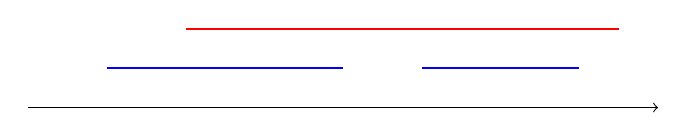
\begin{tikzpicture}
      \draw[->] (0,0) -- (8,0);

      \draw[thick, blue] (1,0.5) -- (4,0.5);
      \draw[thick, red] (2,1) -- (7.5,1);
      \draw[thick, blue] (5,0.5) -- (7,0.5);
    \end{tikzpicture}
    \end{center}
  \end{enumerate}
\end{frame}
\begin{frame}{Q4}
  \begin{enumerate}
    \item [3.] Choose the shortest activity $a$, discard all activities overlapping with $a$ and recurse. Incorrect: 
    \vspace{0.5cm}
    \begin{center}
    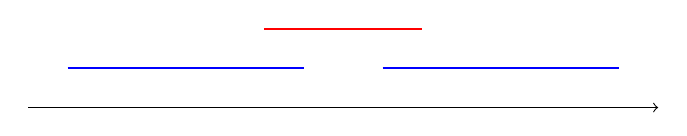
\begin{tikzpicture}
      \draw[->] (0,0) -- (8,0);

      \draw[thick, blue] (0.5,0.5) -- (3.5,0.5);
      \draw[thick, red] (3,1) -- (5,1);
      \draw[thick, blue] (4.5,0.5) -- (7.5,0.5);
    \end{tikzpicture}
    \end{center}
    \vspace{0.5cm}
    \item [4.] (Bonus, not in tutorial) Choose activity $a$ that overlaps with the least number of activities. Incorrect, but it is not as easy to find a counterexample with one activity with the strictly least number of overlapping activities. See last page of slide for an answer. 
    \par This shows the importance of proving that your greedy strategy is correct. 
  \end{enumerate}
  
\end{frame}
\begin{frame}{Q5}
  Now we devise and prove a greedy algorithm based on the idea in Q4(a). 
  \par Optimal substructure: let $S$ be an optimal schedule containing an activity $a$. Then $S$ induces an optimal schedule for the subset of activities that end before start of $a$, as well as an optimal schedule for the subset of activities that start after end of $a$ (otherwise, there will be contradiction). 
  \par Greedy choice property: any optimal schedule $S$ induces via swap/exchange argument an optimal schedule containing the activity $a^*$ that starts last (globally). This is because there is no harm swapping $a^*$ with the activity $a$ starting last among activities in $S$. 
  \par The algorithm is an obvious implementation of the idea (start by sorting start times). 
\end{frame}
\begin{frame}{Bonus}
  \vspace{0.5cm}
    \begin{center}
    \begin{tikzpicture}
      \draw[->] (0,0) -- (8,0);

      \draw[thick, blue] (1,0.5) -- (2,0.5);
      \draw[thick, blue] (2.5,0.5) -- (3.5,0.5);
      \draw[thick, blue] (4,0.5) -- (5,0.5);
      \draw[thick, blue] (5.5,0.5) -- (6.5,0.5);
      \draw[thick, black] (1.75,1) -- (2.75,1);
      \draw[thick, red] (3.25,1) -- (4.25,1);
      \draw[thick, black] (4.75,1) -- (5.75,1);
      \draw[thick, black] (1.75,1.5) -- (2.75,1.5);
      \draw[thick, black] (1.75,2) -- (2.75,2);
      \draw[thick, black] (4.75,1.5) -- (5.75,1.5);
      \draw[thick, black] (4.75,2) -- (5.75,2);
    \end{tikzpicture}
    \end{center}
\end{frame}
\end{document}
